\section{The circle $|x|^2=2$}\label{sec:circle}

The two uncolorable alphabets $\{0,\pm1,\pm\sqrt2\}$ and $\{0,\pm1,\pm\sqrt{-2}\}$ both have
$|x|^2=2$, and in both the conjugate $x^{*}=\pm x$ is already a letter.  For a general complex
$x$ the alphabet that is closed under conjugation is
\[
\mathcal A(x)=\{0,\pm1,\pm x,\pm x^{*}\},\qquad P(x)=S(\mathcal A(x)).
\]
For generic $x$ the pool $P(x)$ has 145 rays; at special $x$ some of them coincide (49 remain
at $x=\sqrt{\pm2}$).  Versions 1--9 used this alphabet at one
point, $x=(1+\sqrt{-7})/2$, found the pool uncolorable, and attributed that to the arithmetic of
the ring of integers of $\Q(\sqrt{-7})$.  It is a property of the whole circle.  This section
proves that (Theorem~\ref{thm:circle}) and then determines every $x$ at which $P(x)$ is
uncolorable (Theorem~\ref{thm:conj}).

\begin{theorem}\label{thm:circle}
Let $W$ be the list of 45 words in Table~\ref{tab:words}.
\begin{enumerate}
\item[(i)] For every $x\in\C$ with $|x|^2=2$ the rays of $W$ form a KS-uncolorable set.
Consequently $P(x)$ is uncolorable for every such~$x$.
\item[(ii)] The orthogonalities among the 145 words that hold for every $x\in\C$ form a colorable
configuration (366 pairs, 22 triads).  Hence $P(x)$ is colorable for every $x$ outside a finite
union of proper real algebraic subsets of~$\C$.
\item[(iii)] No list of fewer than 45 of the 145 words is uncolorable by virtue of the
orthogonalities that hold along the whole circle.  Consequently no fixed list of fewer than 45
words over $\mathcal A(x)$ is uncolorable at every point of the circle.
\end{enumerate}
Part~(iii) concerns fixed lists of words over this alphabet.  It says nothing about other
parametrized families of KS sets.
\end{theorem}

\begin{proof}
The inner product of two words is a polynomial in $x$ and $x^{*}$ with integer coefficients, of
degree at most~2.

(i)  On the circle, $xx^{*}=2$ reduces every such polynomial to an integer combination of
$1,x,x^{*},x^2,x^{*2}$.  With $x=\sqrt2e^{i\theta}$ these are constant multiples of
$e^{ik\theta}$, $k=0,\pm1,\pm2$, which are linearly independent functions of~$\theta$.  So an
inner product vanishes at every point of the circle if and only if every reduced coefficient is
zero, a finite check in integers.  It yields 98 pairs among the words of $W$ that are orthogonal
at every point of the circle, forming the 22 triads listed in Appendix~\ref{app:triads}.  A SAT
solver shows that the configuration with these 98 exclusions and 22 triads has no coloring.  Now
fix $x$ on the circle.  If the 45 words give 45 distinct rays, the orthogonality graph at $x$
contains the 98 pairs, and any further pairs or triads only add constraints, so there is no
coloring.  If two words give the same ray, a coloring at $x$ assigns them the same value and so
would also be a coloring of the 45-vertex configuration; there is none.  (Two words that are
orthogonal for every $x$ on the circle cannot coincide at any point of it.)

(ii)  Without the relation, the monomials $x^ax^{*b}$ are linearly independent functions
on~$\C$, so an inner product vanishes for all $x$ iff all its coefficients vanish.  This yields
366 pairs and 22 triads on the 145 words, and a SAT solver finds a coloring.  Each remaining
inner product is a nonzero polynomial in $x,x^{*}$ and vanishes only on a proper real algebraic
subset.  For each pair of the 145 words at least one $2\times2$ minor of the pair is a nonzero
polynomial, so the set of $x$ at which the two words give the same ray is also a proper real
algebraic subset.  Away from those finitely many subsets the 145 rays are distinct, no further
pair is orthogonal, and the coloring found is a coloring of $P(x)$.

(iii)  The 145 words with the pairs and triads that hold along the whole circle (378 pairs, 34
triads) form a finite configuration, and the certifier of Section~\ref{sec:methods} returns 45 as
its minimum, with a certificate of 408 colorable sets.  For the consequence: the exceptional
points of the circle, at which some further inner product vanishes or two words coincide, are
finite in number, since each such condition is a nonzero trigonometric polynomial in~$\theta$.
A list uncolorable at every point of the circle is uncolorable at a non-exceptional point, where
the configuration is exactly the one just described.

The script \texttt{ks\_modulus2\_circle.py} carries out all three computations.  Its
output file, \texttt{results/modulus2\_circle.json}, holds the 145 words, both graphs, the
coloring of part~(ii) and the certificate of part~(iii).
\end{proof}

\begin{table}[t]
\centering
\caption{The 45 words of Theorem~\ref{thm:circle}.  A bar is a minus sign and $x^{*}$ is the
complex conjugate, so $\bar x^{*}=-x^{*}$.  The list is one minimum set; we have not enumerated
the others.}
\label{tab:words}
\small
\begin{tabular}{rl@{\qquad}rl@{\qquad}rl@{\qquad}rl@{\qquad}rl}
\hline
1 & $0\,0\,1$ & 10 & $1\,0\,1$ & 19 & $1\,1\,x^{*}$ & 28 & $1\,x^{*}\,\bar 1$ & 37 & $x\,\bar 1\,0$ \\
2 & $0\,1\,0$ & 11 & $1\,0\,\bar 1$ & 20 & $1\,1\,\bar x^{*}$ & 29 & $1\,\bar x^{*}\,0$ & 38 & $x\,\bar 1\,1$ \\
3 & $0\,1\,1$ & 12 & $1\,0\,x$ & 21 & $1\,\bar 1\,0$ & 30 & $1\,\bar x^{*}\,1$ & 39 & $x\,\bar 1\,\bar 1$ \\
4 & $0\,1\,\bar 1$ & 13 & $1\,0\,\bar x$ & 22 & $1\,\bar 1\,x$ & 31 & $1\,\bar x^{*}\,\bar 1$ & 40 & $x^{*}\,0\,1$ \\
5 & $0\,1\,x$ & 14 & $1\,0\,x^{*}$ & 23 & $1\,\bar 1\,\bar x$ & 32 & $x\,0\,1$ & 41 & $x^{*}\,0\,\bar 1$ \\
6 & $0\,1\,\bar x$ & 15 & $1\,0\,\bar x^{*}$ & 24 & $1\,\bar 1\,x^{*}$ & 33 & $x\,0\,\bar 1$ & 42 & $x^{*}\,1\,1$ \\
7 & $0\,x^{*}\,1$ & 16 & $1\,1\,0$ & 25 & $1\,\bar 1\,\bar x^{*}$ & 34 & $x\,1\,0$ & 43 & $x^{*}\,1\,\bar 1$ \\
8 & $0\,x^{*}\,\bar 1$ & 17 & $1\,1\,x$ & 26 & $1\,x^{*}\,0$ & 35 & $x\,1\,1$ & 44 & $x^{*}\,\bar 1\,1$ \\
9 & $1\,0\,0$ & 18 & $1\,1\,\bar x$ & 27 & $1\,x^{*}\,1$ & 36 & $x\,1\,\bar 1$ & 45 & $x^{*}\,\bar 1\,\bar 1$ \\
\hline
\end{tabular}

\end{table}

Comparing (i) and (ii): of the 378 pairs present along the circle, 366 are present for every
$x$, and the other 12 are all of the form $1+1-x^{*}x=0$, as in
$(x,1,1)\perp(x,\bar1,\bar1)$.  With them come 12 further triads.  These 12 pairs are the
difference between a colorable pool and an uncolorable one, and the relation behind them is the
one Peres's cube uses at $x=\sqrt2$ (Fig.~\ref{fig:generic}).

\begin{corollary}\label{cor:points}
\begin{enumerate}
\item[(a)] At $x=\sqrt2$ and at $x=\sqrt{-2}$ the 45 words give exactly 33 distinct rays.  By
Computed fact~\ref{fact:peres} these are the unique minimum sets of those pools; at $x=\sqrt2$
they are the 33 rays of Peres.
\item[(b)] At $x=(1+\sqrt{-7})/2$, $P(x)$ is the 145-ray pool studied in earlier versions.  It is
uncolorable because $|x|^2=2$.
\item[(c)] The words $(1,1,x)$ and $(1,0,x^{*})$ of $W$ have squared overlap
$|1+x^{*2}|^2/12=(5+4\cos2\theta)/12$, which is not constant.  The sets of part~(i) are therefore
not all unitarily equivalent: the multiset of squared overlaps between rays is a unitary
invariant that does not depend on labelling, and it takes infinitely many values along the
circle.
\item[(d)] At $x=(1+\sqrt{-7})/2$ the 45 words give 45 distinct rays with 114 orthogonal pairs
and 26 triads, and this set contains a 43-ray KS subset; 43 is the certified minimum within it.
\end{enumerate}
\end{corollary}

\begin{figure}[t]
\centering
\begin{tikzpicture}[scale=1.55]
\draw[->,gray] (-2.45,0) -- (2.6,0) node[right] {$\mathrm{Re}\,x$};
\draw[->,gray] (0,-2.1) -- (0,2.25) node[above] {$\mathrm{Im}\,x$};
\foreach \t in {30,60,120,150} \draw[line width=0.9pt] (\t:-1.9) -- (\t:1.9);
\draw[line width=0.9pt] (0,0) circle (1.4142);
\draw[line width=0.9pt] (0,0) circle (0.7071);
\foreach \p in {-2,-0.5,0.5,2} \fill (\p,0) circle (0.05);
\draw[fill=white,line width=0.5pt] (0,0) circle (0.06);
\node[font=\small,anchor=south] at (2,0.08) {$2$: $\CK$};
\fill (1.4142,0) circle (0.05) node[below right,font=\small] {$\sqrt2$: Peres};
\fill (0,1.4142) circle (0.05);
\node[font=\small,anchor=south west] at (0.08,1.78) {$\sqrt{-2}$: 33 rays};
\draw[gray,line width=0.3pt] (0.03,1.46) -- (0.12,1.8);
\fill (0.5,1.3229) circle (0.05);
\node[font=\small,anchor=west] at (1.2,1.45) {$\tfrac{1+\sqrt{-7}}{2}$: minimum 43};
\draw[gray,line width=0.3pt] (0.55,1.34) -- (1.18,1.44);
\node[font=\small,anchor=east] at (-1.25,1.5) {$|x|^2=2$};
\node[font=\small,anchor=east] at (-1.75,-0.5) {$|x|^2=\tfrac12$};
\draw[gray,line width=0.3pt] (-0.69,-0.17) -- (-1.73,-0.48);
\node[font=\small,anchor=west] at (1.68,-0.97) {$\arg x=-30^\circ$};
\node[font=\small,anchor=north west] at (0.97,-1.66) {$\arg x=-60^\circ$};
\node[font=\small,align=left,anchor=north east] at (-1.2,-1.5) {elsewhere:\\colorable};
\end{tikzpicture}
\caption{The alphabet $\{0,\pm1,\pm x,\pm x^{*}\}$.  Its pool is uncolorable exactly on the set
drawn in black: the circles $|x|^2=2$ and $|x|^2=\tfrac12$, the four lines through the origin at
$\pm30^\circ$ and $\pm60^\circ$ to the real axis with the origin removed, and the points
$\pm2,\pm\tfrac12$ (Theorem~\ref{thm:conj}).  The pool is unchanged by $x\mapsto-x$ and
$x\mapsto x^{*}$, so one quadrant suffices.  At the four axis points of the outer circle, which
are two alphabets up to sign, the 45 words of Table~\ref{tab:words} collapse to 33 rays.  At $(1+\sqrt{-7})/2$ the additional
relation $x+x^{*}=1$ adds orthogonalities and the minimum drops from 45 to~43.}
\label{fig:circle}
\end{figure}

\subsection{The point $x=(1+\sqrt{-7})/2$}

Let $\alpha=(1+\sqrt{-7})/2$, so $|\alpha|^2=2$ and $\alpha+\alpha^{*}=1$.

\begin{fact}[The $\Q(\sqrt{-7})$ pool]\label{fact:heegner}
$P(\alpha)$ has 145 rays, 522 orthogonal pairs and 42 triads, against 378 and 34 at a generic
point of the circle.  Its minimum uncolorable subsets have 43 rays, certified.  There are exactly
six of them, in two orbits under signed permutations of the coordinates, each with 23 bases; the
one we use has 107 pairs and degree sequence $4^{16}5^{20}6^{4}8^{2}10^{1}$.  The completed pool
has 685 rays, 1746 pairs and 582 triads; its minimum is \heegnercompletedmin.
\end{fact}

So the additional relation at this point is worth two rays: 43 against 45
(Corollary~\ref{cor:points}d).  It is the pools $P(x)$ that form a continuous family through
this point.  Theorem~\ref{thm:circle} proves that $P(\alpha)$ is uncolorable; that its minimum is
43 is a separate computation.

Table~\ref{tab:heegner} puts this point in the setting in which earlier versions found it.  For
each of the nine imaginary quadratic fields of class number one we take the generator $a$ of the
ring of integers and the alphabet $\{0,\pm1,\pm a,\pm a^{*}\}$.  The uncolorable rows are
$d=2$ (a point of the circle), $d=3$ (the roots-of-unity alphabet $S_6$ of
Theorem~\ref{thm:6n}) and $d=7$ (a point of the circle).  Class number plays no role that we can
see; Theorems~\ref{thm:6n} and~\ref{thm:circle} account for all three rows.

\begin{table}[t]
\centering
\caption{Raw pools of $\{0,\pm1,\pm a,\pm a^{*}\}$, $a$ the generator of the ring of integers of
$\Q(\sqrt{-d})$: $a=\sqrt{-d}$ for $d=1,2$ and $a=(1+\sqrt{-d})/2$ otherwise.  Minima are
certified.  For $d=1$ version~9 printed a different, larger alphabet in this row; see the text.}
\label{tab:heegner}
\begin{tabular}{rcrrrcc}
\toprule
$d$ & $|a|^2$ & Rays & Pairs & Triads & Colorable & Min \\
\midrule
1 & 1 & 31 & 69 & 7 & yes & --- \\
2 & 2 & 49 & 120 & 16 & \textbf{no} & \textbf{33} \\
3 & 1 & 57 & 174 & 22 & \textbf{no} & \textbf{33} \\
7 & 2 & 145 & 522 & 42 & \textbf{no} & \textbf{43} \\
11, 19, 43, 67, 163 & $3,5,11,17,41$ & 145 & 462 & 30 & yes & --- \\
\bottomrule
\end{tabular}
\end{table}

For $d=1$ the letters are $0,\pm1,\pm i$ and the pool is $S_4$, colorable by
Theorem~\ref{thm:6n}.  The larger Gaussian alphabet $\{0,\pm1,\pm i,\pm(1+i)\}$, which contains
the element $1+i$ of squared modulus~2, generates 127 rays, 465 pairs and 51 triads; that pool is
uncolorable with certified minimum~33 (16 bases in the set found).

\subsection{Relation to the family of Gould and Aravind}

Gould and Aravind~\cite{GouldAravind2010} exhibited a family of 33-ray sets with the
orthogonality graph of Peres's set, depending on three phases, containing the sets of Peres and
of Penrose; Flores Gordillo~\cite{FloresGordillo2026} reports that after removing diagonal
unitaries the family is a circle (we have not audited that proof).  That family is different from the one in
Theorem~\ref{thm:circle}.  Its members have 33 rays and a constant graph.  Ours has 45 rays at a
generic point and cannot contain a 33-ray KS set there: every orthogonality of $P(x)$ at a generic
point of the circle is also one of $P(\alpha)$, whose minimum is~43, so no subset of $P(x)$ with
fewer than 43 rays is uncolorable.  (Theorem~\ref{thm:conj} below gives 45.)  The two families meet at $x=\sqrt2$, where both give Peres's
set.  We have not found the family of Theorem~\ref{thm:circle} in the literature, but we have not
made a systematic search and make no claim of priority.

\subsection{Every conjugate-closed alphabet}\label{sec:conjclosed}

Theorem~\ref{thm:circle} settles one curve in the plane of~$x$.  The method of
Theorem~\ref{thm:twosymbol} settles the plane.

\begin{theorem}[Conjugate-closed alphabets]\label{thm:conj}
Let $x$ be a nonzero complex number and $P(x)$ the pool of all words over
$\{0,\pm1,\pm x,\pm x^{*}\}$.
\begin{enumerate}[label=(\roman*)]
\item $P(x)$ is uncolorable if and only if one of the following holds:
\begin{enumerate}[label=(\alph*)]
\item $|x|^2=2$;
\item $|x|^2=\tfrac12$;
\item $x^{*}/x$ is a primitive third or sixth root of unity, that is, $\arg x$ is one of
$\pm30^\circ$, $\pm60^\circ$, $\pm120^\circ$, $\pm150^\circ$;
\item $x\in\{\pm2,\pm\tfrac12\}$.
\end{enumerate}
\item At every point of the curves (a)--(c) other than the special points of
Table~\ref{tab:conj}, the minimum uncolorable subset of $P(x)$ has 45 rays on $|x|^2=2$ and 33
rays on $|x|^2=\tfrac12$ and on the four lines of~(c).  At the special points the minima are
those of Table~\ref{tab:conj}; two of them are bounds and not certified values.
\item For every $x$ other than $\pm1\pm i$, no uncolorable subset of $P(x)$ has fewer than 31
rays, and 31 is attained at $x=\pm2,\pm\tfrac12$, where $P(x)$ is the integer pool.  At
$x=\pm1\pm i$ the pool is uncolorable and we have not established the bound 31; there the
minimum lies between the general lower bound 24 and~45.
\end{enumerate}
\end{theorem}

\begin{proof}
The argument is that of Theorem~\ref{thm:twosymbol} with two more monomials.  An inner product of
two words, and a $2\times2$ minor of two words, is an integer combination
\[
c_0+c_1x+c_2x^{*}+c_3|x|^2+c_4x^2+c_5x^{*2}
\]
with $\sum|c_k|\le3$; 376 nonzero coefficient vectors occur.  With $x=a+ib$ the combination
vanishes when
\[
b\,\bigl[(c_1-c_2)+2(c_4-c_5)\,a\bigr]=0,\qquad
c_0+(c_1+c_2)\,a+(c_3+c_4+c_5)\,a^2+(c_3-c_4-c_5)\,b^2=0 .
\]
Both conditions involve $b$ only through the factor $b$ and through $b^2$, and the second is
linear in~$b^2$.  The solution set of one vector is therefore made up of finitely many points
and of whole curves of three kinds: the real axis, a vertical line, and a curve
$b^2=g_0+g_1a+g_2a^2$.  We work throughout in the coordinates $(a,b^2)$, which identifies $x$
with $x^{*}$; this loses nothing, because $P(x^{*})=P(x)$.  Two different curves of these kinds
meet in at most two values of~$a$.  A vector that vanishes at infinitely many points of a curve
$b^2=g(a)$ with $b\ne0$ vanishes on all of it: the first condition then forces
$(c_1-c_2)+2(c_4-c_5)a$ to be identically zero, and substituting $b^2=g(a)$ in the second
gives a polynomial in $a$ with infinitely many roots.  So the two lines of a pair such as
$b^2=3a^2$, and the two branches of a hyperbola, need not be treated separately.
Going through the 376 vectors gives fourteen curves with points other than the origin:
\[
\mathrm{Im}\,x=0,\quad \mathrm{Re}\,x=0,\ \pm\tfrac12,\quad |x|^2=\tfrac12,\ 1,\ 2,\quad
|x\pm1|=1,\quad \mathrm{Re}\,x^2=0,\ \pm\tfrac12,\quad x^2+x^{*2}=\pm|x|^2 .
\]
The last two are the pairs of lines $b^2=a^2/3$ and $b^2=3a^2$ of part~(c).  Call a nonzero point
\emph{special} if it is an isolated solution of some vector or lies on two of the curves; there
are 53 special points with $\mathrm{Im}\,x\ge0$ (92 in the plane, 14 of them real).  As in Theorem~\ref{thm:twosymbol}, the set of vectors that vanish at $x$,
and with it the list of coinciding words and the orthogonality graph of $P(x)$, is the same at
all points on no curve, and the same at all non-special points of any one curve.  That leaves
$1+14+53=68$ cases.  The pool is also unchanged by $x\mapsto-x$, which reduces
the special points to 28 classes and the curves to 12; unlike the two-symbol pool it is not
unchanged by $x\mapsto1/x$.

The script \texttt{ks\_conjugate\_closed\_theorem.py} lists the curves and the special points in
exact arithmetic ($a$ and $b^2$ in one quadratic field $\Q(\sqrt d)$), builds the 68 graphs, decides colorability of
each, and runs the certification procedure of Section~\ref{sec:methods} on the uncolorable ones.
Table~\ref{tab:conj} is the result.  The uncolorable cases are the curves (a), (b) and (c), every
special point on them, and the points $\pm2,\pm\tfrac12$; all other cases are colorable.  That
is~(i).  Part~(ii) is the corresponding rows of the table.  For~(iii), the certifier terminated
with a minimum of at least 31 in every uncolorable case except four.  For those four we made
separate runs, each of which only decides whether an uncolorable subset of fewer than a given
number of rays exists.  At $\eta/\sqrt2$ and at $2\zeta$
(notation of Table~\ref{tab:conj}) there is none of fewer than 33 rays,
which with the 33-ray sets found makes 33 the minimum.  At $\zeta/\sqrt2$ there is none of
fewer than 32, and the run for 33 did not terminate in eight hours.  At $x=\pm1\pm i$ the run
for 31 did not terminate in eight hours.  The
witnesses are archived; the lists of colorable sets produced by these runs are not, so the
lower bounds of this theorem can be reproduced only by rerunning the script.

Part~(c) also has a proof that needs no new computation.  A word whose nonzero entries are all
$\pm x$ or $\pm x^{*}$ is $x$ times a word over $\{0,\pm1,\pm u\}$ with $u=x^{*}/x$, so $P(x)$
contains every ray of the two-symbol pool $S(u)$.  By Theorem~\ref{thm:twosymbol}, $S(u)$ is
uncolorable when $u$ is a primitive third or sixth root of unity, with a 33-ray minimum set
having the graph of the Eisenstein set, and Lemma~\ref{lem:restrict} carries this to $P(x)$.
This argument gives nothing more, since $S(u)$ is colorable for every other $u$ on the unit
circle.
\end{proof}

\begin{table}[t]
\centering
\caption{Every pool of the conjugate-closed alphabet $\{0,\pm1,\pm x,\pm x^{*}\}$
(Theorem~\ref{thm:conj}).  A curve stands for its points other than the special points listed
below it, and each special point stands for its images under $x\mapsto-x$ and
$x\mapsto x^{*}$.  $\zeta=e^{i\pi/3}$, $\eta=e^{i\pi/6}$, $\varphi=(1+\sqrt5)/2$.  ``Min'' is
the certified size of the smallest uncolorable subset; ``32--33'' means that 33 rays suffice
and fewer than 32 do not; ``$\le45$'' is an upper bound only.  The last column gives the graph
of the smallest set found (isomorphism by VF2).}
\label{tab:conj}
\small
\begin{tabular}{@{}lrrrcl@{}}
\toprule
$x$ & Rays & Pairs & Triads & Min & Smallest set found \\
\midrule
on no curve & 145 & 366 & 22 & --- & colorable \\
$\mathrm{Im}\,x=0$;\ \ $\mathrm{Re}\,x=0$ & 49 & 114 & 10 & --- & colorable \\
$|x|=1$ & 109 & 276 & 16 & --- & colorable \\
$\mathrm{Re}\,x^2=0$ & 127 & 321 & 19 & --- & colorable \\
$\mathrm{Re}\,x=\pm\tfrac12$;\ \ $|x\pm1|=1$ & 145 & 462 & 30 & --- & colorable \\
$\mathrm{Re}\,x^2=\pm\tfrac12$ & 145 & 378 & 22 & --- & colorable \\
$|x|^2=2$ & 145 & 378 & 34 & \textbf{45} & 45 rays, 98 pairs \\
$|x|^2=\tfrac12$ & 145 & 390 & 46 & \textbf{33} & Peres \\
$\arg x=\pm30^\circ,\pm60^\circ,\pm120^\circ,\pm150^\circ$ & 145 & 390 & 30 & \textbf{33} & Eisenstein 33 \\
\midrule
$1$ & 13 & 24 & 4 & --- & colorable \\
$i$ & 31 & 69 & 7 & --- & colorable \\
$\varphi,\ 1/\varphi$ & 49 & 138 & 10 & --- & colorable \\
$e^{i\pi/4}$ & 91 & 231 & 13 & --- & colorable \\
$|x-1|=1$ and $\mathrm{Re}\,x^2=\tfrac12$ & 145 & 474 & 30 & --- & colorable \\
\midrule
$2,\ \tfrac12$ & 49 & 138 & 26 & \textbf{31} & $\CK$ \\
$\sqrt2,\ 1/\sqrt2,\ \sqrt{-2},\ 1/\sqrt{-2}$ & 49 & 120 & 16 & \textbf{33} & Peres \\
$(1+i)/2$ & 127 & 465 & 51 & \textbf{33} & Peres \\
$(1+\sqrt{-7})/4$ & 145 & 486 & 54 & \textbf{33} & Peres \\
$\eta/\sqrt2$ & 145 & 414 & 54 & \textbf{33} & Peres \\
$\zeta/\sqrt2$ & 145 & 414 & 54 & 32--33 & Peres \\
$\zeta$ & 57 & 174 & 22 & \textbf{33} & Eisenstein 33 \\
$\eta$ & 109 & 312 & 24 & \textbf{33} & Eisenstein 33 \\
$\zeta/2$ & 145 & 414 & 54 & \textbf{33} & Eisenstein 33 \\
$\eta/\sqrt3,\ \sqrt3\,\eta$ & 145 & 486 & 38 & \textbf{33} & Eisenstein 33 \\
$\sqrt2\,\eta,\ \sqrt2\,\zeta$ & 145 & 402 & 42 & \textbf{33} & Eisenstein 33 \\
$2\zeta$ & 145 & 438 & 62 & \textbf{33} & Eisenstein 33 \\
$(1+\sqrt{-7})/2$ & 145 & 522 & 42 & \textbf{43} & 43 rays, 107 pairs \\
$(\sqrt5+\sqrt{-3})/2,\ (\sqrt3+\sqrt{-5})/2$ & 145 & 390 & 34 & \textbf{45} & 45 rays, 98 pairs \\
$1+i$ & 127 & 477 & 63 & $\le45$ & 45 rays, 98 pairs \\
\bottomrule
\end{tabular}
\end{table}

Five remarks.

First, the theorem contains the statement of Theorem~\ref{thm:circle}(i) that $P(x)$ is
uncolorable on the circle, and sharpens the conclusion of~(ii): the
``finite union of proper real algebraic subsets'' outside which $P(x)$ is colorable is two
circles, four lines without the origin, and four points.  It does not replace part~(iii) or the explicit list of
words, and the proof of Theorem~\ref{thm:circle}(i) by a fixed list remains the reason the
circle is uncolorable.

Second, the three curves behave differently.  On $|x|^2=2$ the minimum is 45 except at
finitely many points.  On $|x|^2=\tfrac12$ it is 33 except possibly at the one class of
points marked 32--33, and the smallest set found has the orthogonality graph of Peres's set at
a generic point and at every special point of that circle.  So $|x|^2=\tfrac12$ carries a
one-parameter family of 33-ray sets with Peres's graph.  We have not compared it with the family
of Gould and Aravind discussed above.  Every point of the lines other than the origin has a
33-ray uncolorable set with the graph of the Eisenstein set of Section~\ref{sec:roots}, written
in the letters $\{0,\pm x,\pm x^{*}\}$, by the last paragraph of the proof; it is a minimum set
wherever the table certifies~33.

Third, the theorem accounts for Table~\ref{tab:heegner} without reference to number fields:
$d=2$ and $d=7$ are points of $|x|^2=2$, $d=3$ is the point $\zeta$ of the $60^\circ$ line, and
for $d=11,19,43,67,163$ the generator lies on $\mathrm{Re}\,x=\tfrac12$ and on no uncolorable
curve.  The row $(1+i)/2$ of Table~\ref{tab:conj} is the Gaussian alphabet
$\{0,\pm1,\pm i,\pm(1+i)\}$ of the previous subsection, after multiplying every letter by $1+i$.

Fourth, the certified minima of Table~\ref{tab:conj} are 31, 33, 43 and 45.  The alphabet with
the conjugate does not give a KS set smaller than that of Conway and Kochen at any point where
the computation finished, and among the certified cases 31 is reached only by the integer pool.
The statement is incomplete at $x=\pm1\pm i$, where the certifier did not terminate, and at the
class marked 32--33, where the minimum is 32 or 33.

Fifth, like Theorem~\ref{thm:twosymbol} this concerns raw pools.  Completed pools are not
covered.

The script asserts agreement with the number-field constructions of
Section~\ref{sec:catalogue} at seven points, at a generic point and on the circle $|x|^2=2$;
we also rebuilt six further cases with those constructions and found the same counts.  The
graphs of the smallest sets are identified by \texttt{ks\_conjugate\_closed\_identify.py}.

\subsection{Rigidity}

Table~\ref{tab:rigidity} reports the number of infinitesimal flexes in $\C^3$ of each minimum
set: the dimension of the null space of the Jacobian of the equations $|v_i|^2=1$,
$\braket{v_i}{v_j}=0$ (one complex equation for each orthogonal pair), minus the $n+8$ dimensions
accounted for by a common unitary and a phase on each vector.  The ranks are numerical; in every
case the smallest retained singular value exceeds $0.2$ and the largest discarded one is below
$2\times10^{-15}$.  Zero flexes, if confirmed by an exact rank computation, means the set is locally rigid.  It does
not by itself mean the
realization is unique up to unitary equivalence; for $\CK$ that stronger statement is the theorem
of Trandafir and Cabello~\cite{TrandafirCabello2025}, and for the Eisenstein set it is asserted by
Cabello~\cite{Cabello2025simplest}.

\begin{table}[t]
\centering
\caption{Infinitesimal flexes in $\C^3$ (numerical ranks).}
\label{tab:rigidity}
\begin{tabular}{lrrrc}
\toprule
Set & Rays & Pairs & $\dim\ker J$ & Flexes \\
\midrule
$\CK$ & 31 & 71 & 39 & 0 \\
Eisenstein, 33 rays & 33 & 78 & 41 & 0 \\
Peres, 33 rays & 33 & 72 & 42 & 1 \\
$\sqrt{-2}$, 33 rays & 33 & 72 & 42 & 1 \\
$\Q(\sqrt{-7})$, 43 rays & 43 & 107 & 51 & 0 \\
Supergolden, 47 rays & 47 & 110 & 55 & 0 \\
Supergolden (completed pool), 47 rays & 47 & 108 & 55 & 0 \\
Golden, 51 rays & 51 & 118 & 59 & 0 \\
Cube root of two, 60 rays & 60 & 144 & 68 & 0 \\
45 words at $\theta=0.3$ and at $\theta=1.0$ & 45 & 98 & 55 & 2 \\
45 words at $x=(1+\sqrt{-7})/2$ & 45 & 114 & 53 & 0 \\
\bottomrule
\end{tabular}
\end{table}

The single flex of the Peres set is the circle of Gould--Aravind and Flores Gordillo, and it is a
genuine deformation, not merely an infinitesimal one.  Versions 1--7 of this paper claimed the
opposite on the strength of a second-order computation that contained an indexing error, found
by Flores Gordillo and corrected in version~8.  The 45 words have two flexes at each of the two phases we computed
($\theta=0.3$ and $\theta=1.0$).  One of them is motion along the circle
(Corollary~\ref{cor:points}c); we have not identified the other.  At $x=(1+\sqrt{-7})/2$, with
the 16 additional orthogonalities imposed, the same 45 rays are numerically infinitesimally
rigid.
